\title{Compilers Engineering 2019\\
Mini Assignment 1: \\
An Introduction to the LLVM Infrastructure, AST,
IR and Compiler Options\\
Report}
\author{Sai Harsha Kottapalli\\CS17BTECH11036}
\date{August 28, 2019}

\documentclass[12pt]{article}
\usepackage{graphicx}
\usepackage[most]{tcolorbox}

\definecolor{bg}{RGB}{220,220,220}

\begin{document}
\maketitle

\section{GCC}
On compilation of source code, gcc usually produces two types of output if it has failed.
One being “errors” and other being “warnings”.
Errors are shown in the format: 
```
bubbleSort(arr, n)

~/bubblesort.cpp: In function ‘int main()’:
~/bubblesort.cpp:38:23: error: expected ‘;’ before ‘cout’
```
where the file’s name, scope(limited to functions), line number, column number and the problem occurred while compilation is shown.
In above example we forgot to put a semi-colon after the statement which gave rise to the associated error.
In the case of Warnings, they are usually the code which might still run during execution but is not what the user might desire.
```
int swap(int *a, int *b) {
    int temp = *a;
    *a = *b;
    *b = temp;
}

bubblesort.cpp: In function ‘int swap(int*, int*)’:
bubblesort.cpp:9:1: warning: no return statement in function returning non-void [-Wreturn-type]
    9 | }
```
Here, though the syntax is same as that of error it always has “warning:” to differentiate from other errors.
Usually most warnings help us find bugs without actually having to debug the entire code to identify it and also helps in writing a dis-ambiguous code.

However internally in gcc, there are three cases: warning, error and fatal (internal error ?).
```
gcc/diagnostic.c
```
The definitions are defined where:
Warnings: “correct according to a language specification but likely to be buggy”.
Error: “ill-formed code”
Fatal: “An error which is severe enough that we make no attempt to continue.”
This file implements “the language independent aspect of diagnostic message module” based on the flags passed for compilation.

For language specific errors they are found in gcc/<lang>/error.c (gcc/c/c-errors.c ?)
For C, it is gcc/error.c
warning function just prints warning in the discussed format and continues.
Error function, prints the error and has a flag set to 1 (have_error) so that the object file is not generated.
Fatal function, just quits at that point which the associated error msg and code.

\section{AST Traversal}
 \textbf{About: }\\
 
 The visitor mechanism to traverse the AST according to the link mentioned in the given pdf, allows us to traverse the nodes of the Clang AST in depth-first search way.\\
This can be verified using "\$ clang-check hello.c -ast-dump" or with the help of the commands listed in the clang documentation (in the link shared in question).\\
From the output, we can infer that the traversal outputs the class-names/variable names with scope resolution with DFS as discussed. Basically, what this means is that of the three core classes of clang, all the "decl"(declaration) classes w.r.t. clang are printed.\\\\
 \textbf{How to: }\\

\begin{itemize}
\item \textbf{FrontendAction}\\
When we provide the required actions, this is responsible for executing those during compilation.\\
The structure is an interface and is predefined , so we only have to follow it and implement \textbf{CreateASTConsumer} under it.
\item \textbf{ASTConsumer}\\
Though this interface has many entry points to start with, since, as of now we only deal with the translation unit. Clang documentation recommends the use of only "HandleTranslationUnit" for all of our usage.
\item \textbf{RecursiveASTVisitor}\\
This is the main interface which is responsible for traversal.\\
Here, we can give the required conditions(by grabbing required details, Ex: \textbf{getQualifiedNameAsString()} for name) to find nodes that we require and then accordingly mark them(using dump() function).\\
We also have the option to continue doing so(return true) or stop when necessary.(return false).\\
If we dump everything by default, we get all the declaration names as it should, because we call dump() (therefore marking it) for all declarations.\\
\item \textbf{ASTContext}\\
On the rare cases where we must use global variable, this information of course wont be present in the nodes.\\
Clang documentation therefore asks us to use \textbf{ASTContext} for this scenario. 
\end{itemize}
 
\section{Error Messages for Handling}
\begin{itemize}
\item \textbf{Where to find: }\\
When we lookup the directory hierarchy in the documentation, it is mentioned about "lib/Support" folder. Upon inspecting we find "ErrorHandling.cpp" inside it.\\
\item \textbf{Assert}\\
Firstly, to use assert, we need to include <cassert> header file.\\
This is really helpful in checking the pre-conditions or assumptions that we have (especially before a loop or function definition).\\
The main advantage is that debugging the code becomes really easy when compared to the code without assert. But there is a trade-off.\\
Using "assert" will increase the program execution time, so it is mostly used as mentioned above.\\
\textbf{Ex:}\\assert(!ErrorHandler \&\& "Error handler already registered!\textbackslash n");\\
assert(!ErrorHandler \&\& "Bad alloc error handler already registered!\textbackslash n");\\
assert(old == nullptr \&\& "new-handler already installed");\\
which are accordingly called w.r.t. later execution using those variables.
Here, we check if there is any error handler being referenced or is null, and accordingly the associated error message is printed.\\
In the docs, it is mentioned that for release build asserts are disabled. This makes sense as there are many reasons.\\
1. More errors/ warnings (referencing something that is not present in user's code).\\
2. User needs to know about associated header files and accordingly install them when it is not really required for most cases.\\
3. Program Behavior is undefined when assertion results in false.\\
Although for worst case scenario if user does trigger some buggy code, "llvm\textunderscore unreachable" takes care of it by either exiting the program or skipping that particular branch of the code.\\
\begin{figure}[ht!]
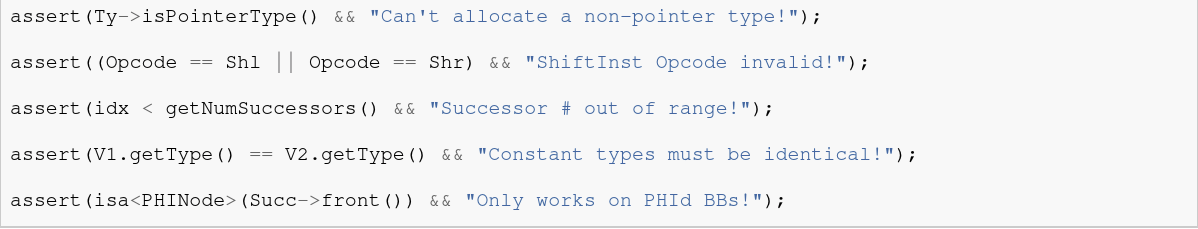
\includegraphics[width=150mm]{3rd.png}
\caption{More examples for assert function}
\end{figure}
\textbf{References:} https://llvm.org/docs/CodingStandards.html
\end{itemize}
 
 \newpage

 
\section {LLVM IR}
\begin{itemize}
\item Sum of two arbitrarily large numbers (no limit no size of the two numbers).
\item Set implementation
\item Generating BST from input pre-order traversal.
\item Binary search iterative
\item Finding BFS and shortest path between two nodes
\item Findings:\\
It is basically a target independent assembly like language which acts as an intermediate representation which an advantage of infinite registers.\\
It is strongly typed.\\
The generated LLVM IR is attached as .ll files.\\
To generate llvm ir from a source code:\\
  \$ clang -S -emit-llvm hello.c\\
\\
source\textunderscore filename gives us the file name and generally ModuleID is same as that.\\
target datalayout is responsible for showing the details of the target system's supported memory layout.\\
$[5$ x $i32]$ implies it is an array of size 5 and of type i32. similarly for n-dimensional arrays.\\
Every function specifies the return type an "(..)" which shows the type of parameters accepted by it.\\
Each function has comments (starts with ;) which specifies the function attributes.\\
\%5, \%6 , etc are register names which are allocated a type using "alloca" and aligned for proper retrieval during memory accesses.\\
We use store keyword when operating and storing data in memory.\\
Most of the ll files is divided into basic blocks(which have no jumps in between them) and can be connected via CFG.\\
A label is present before each of these basic blocks for identifying which block has to be accessed next during the execution flow(jumps are made with the help of "br").\\
Therefore, Label's use is to branch out.\\
"load" is to get data from main memory and store it in register.\\
"preds" tell us which basic block might call the current basic block.
llvm also has struct data type which stores the data types declared inside it.\\
All functions referenced via header files are defined using "declare" keyword in ll file.\\
Phi node is special instruction which chooses a value based on it's pred during the flow.\\
"sext" is used for type casting but both values should be of the integer class/family.\\
"call" is used to call a function with its type and name.\\
Documentation also mentions that IR is static single assignment which means that all variables are declared before use and allocated only once.\\
\end{itemize}

\section {Assembly language:}
\begin{itemize}
\item Name Mangling\\
It can be the case that, when linker is trying link programs in a language, there are functions with same names. In these cases, there would be a conflict.\\
Hence, as a precaution a unique name is chosen for each function, and these unique names are called name mangling.\\
Example: When we declare a variable in different scope or when we overload + symbol for string addition as well as mathematic addition, etc.\\
For the trivial program, there is a "\textunderscore Z1" prepended.\\
When compared with other programs, we can infer that "\textunderscore Z" is prepended as a convention and the number signifies the scope of the variable.\\
For classes, it prepended "\textunderscore ZN"\\
Examples: On redeclaring functions: \textunderscore Z4def1v and \textunderscore Z4def2i.

\end{itemize}

\section {Compiler toolchain and options:}
compiling cpp files with clang - \$ clang++ -Wall -std=c++11 test.cc -o test.\\
-Wall prints warning messages while compiling.\\
llvm-ar: archiving llvm bitcode files.\\
llvm-as: assembler for transformation of human readable LLVM assembly to LLVM bitcode.\\
llvm-dis: opposite to llvm-as, bitcode to human readable assembly.\\
llvm-link: linking multiple llvm modules\\
lli: llvm interpreter for bitcode\\
llc: bitcode to native assembly\\
opt: Apply transformations on bitcode to generate a optimized verion of the input bitcode.(can pass different levels -O{1,2,3,4}).\\
Here, -O0 is no optimization(fastest) and easier to debug.
from {1,2,3} the time taken increases while the optimization level applied also increases.\\
We notice though optimized larger code is generated some times.\\
-std= : to provide a standard for compiling in that particular standard.\\
-arch for providing architechture.\\
-fsyntax-only : just check correctness\\
For most of the programs, the number of resultant basic blocks decreased when optimization was applied.
llvm-diff for differences in files. Example when compared for .ll files, it shows where the functions existed (only left module or only right module).\\

References: https://llvm.org/docs/GettingStarted.html

\section {Kaleidoscope}
Only double type is supported(advantage being types need not be passed).\\
arrays, structs, vectors, etc are supported.\\
global variables are supported but need to make an instance of GlobalVariable class.\\
Supports Accurate Garbage Collection.\\
debugger support is present\\
Docs claim - object orientation, generics, database access, complex numbers, geometric programming.\\
Target Independence.\\
It has an IRBuilder class which tracks the position to insert instructions.\\

References: http://llvm.org/docs/tutorial/index.html
\end{document}